\hypertarget{_g_b_tile_view_8cpp}{}\section{C\+:/\+Users/sjh13/sources/\+Visual\+Boy\+Advance/src/win32/\+G\+B\+Tile\+View.cpp 파일 참조}
\label{_g_b_tile_view_8cpp}\index{C\+:/\+Users/sjh13/sources/\+Visual\+Boy\+Advance/src/win32/\+G\+B\+Tile\+View.\+cpp@{C\+:/\+Users/sjh13/sources/\+Visual\+Boy\+Advance/src/win32/\+G\+B\+Tile\+View.\+cpp}}
{\ttfamily \#include \char`\"{}stdafx.\+h\char`\"{}}\newline
{\ttfamily \#include \char`\"{}vba.\+h\char`\"{}}\newline
{\ttfamily \#include \char`\"{}File\+Dlg.\+h\char`\"{}}\newline
{\ttfamily \#include \char`\"{}G\+B\+Tile\+View.\+h\char`\"{}}\newline
{\ttfamily \#include \char`\"{}Reg.\+h\char`\"{}}\newline
{\ttfamily \#include \char`\"{}Win\+Res\+Util.\+h\char`\"{}}\newline
{\ttfamily \#include \char`\"{}../\+System.\+h\char`\"{}}\newline
{\ttfamily \#include \char`\"{}../\+N\+L\+S.\+h\char`\"{}}\newline
{\ttfamily \#include \char`\"{}../\+Util.\+h\char`\"{}}\newline
{\ttfamily \#include \char`\"{}../gb/gb\+Globals.\+h\char`\"{}}\newline
{\ttfamily \#include $<$png.\+h$>$}\newline
G\+B\+Tile\+View.\+cpp에 대한 include 의존 그래프
\nopagebreak
\begin{figure}[H]
\begin{center}
\leavevmode
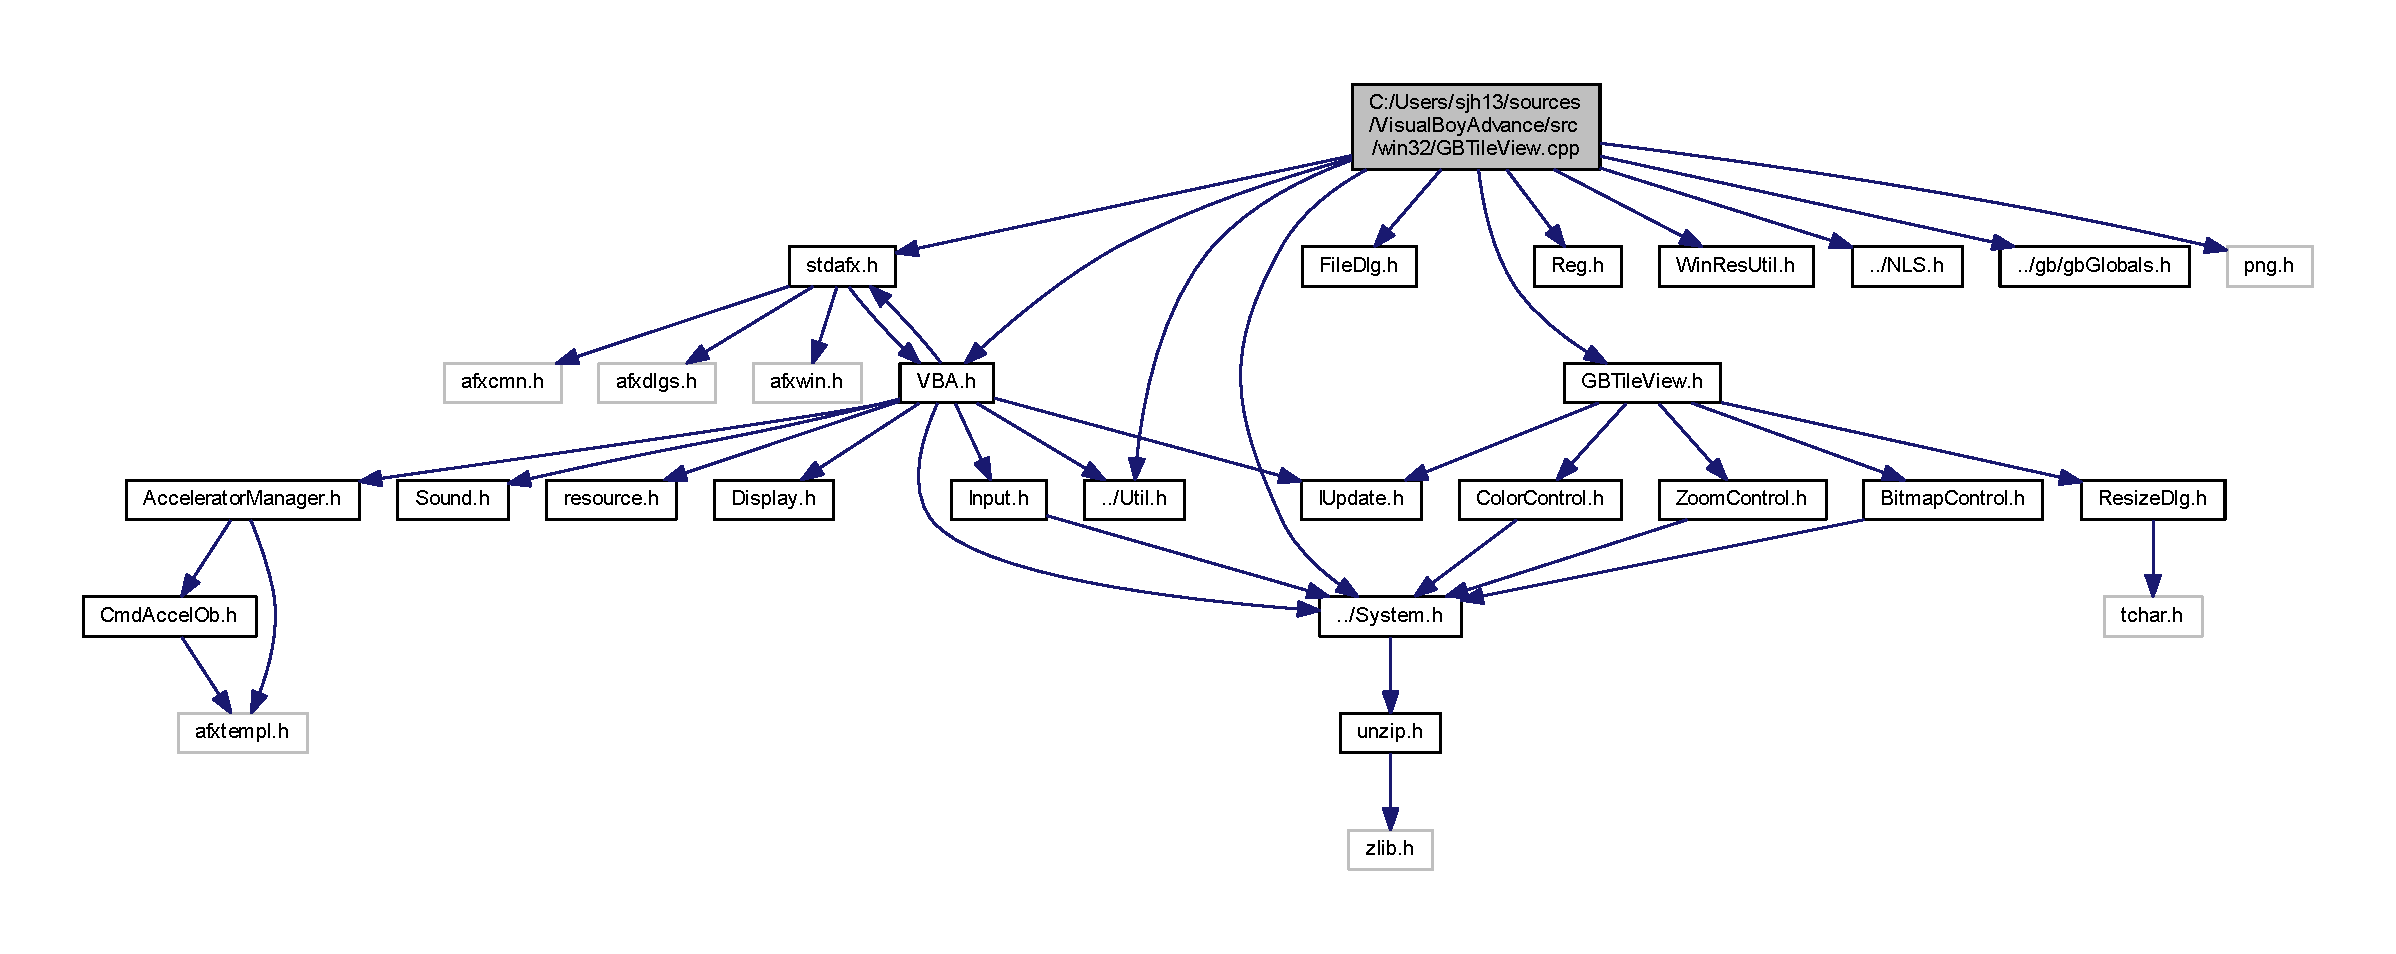
\includegraphics[width=350pt]{_g_b_tile_view_8cpp__incl}
\end{center}
\end{figure}
